% Tiene dos configuraciones extras: "twoside", para diferenciar las páginas pares de las impares, y "marginnote", para poder activar las notas al margen.
\documentclass[marginnote,twoside]{notebookFMG}
% \documentclass[]{book}

\usepackage{lipsum}
% Paquete de creación propia. Carga los entornos de los teoremas. Tiene la opción de mostrar colores en el nombre del teorema, si es que se le entrega la opción de "color".
\usepackage[color]{pkg/theoremenvFMG}
%Options: Sonny, Lenny, Glenn, Conny, Rejne, Bjarne, Bjornstrup
\usepackage[Lenny]{fncychap}

%% Datos de la portada
\def\tituloportada {Nuevo Titulo de la Portada}
\def\autordeldocumento {Francisco Muñoz Guajardo}
\def\repositorio {github.com/LaTeX-pm/Template-Apuntes}
\def\fecha {\today}
\def\nombredelcurso {Curso ultra bkn}
\def\codigodelcurso {CO-1234}
\def\nombreuniversidad {Universidad de Chile}
\def\nombrefacultad {Facultad de Ciencias Físicas y Matemáticas}
\def\departamentouniversidad {Departamento de la Universidad}

% Si se desea cambiar la tabla de la portada
\renewcommand{\tablaautor}{
    \begin{tabular}{ll}
        Autor: & \autordeldocumento \\
        Repositorio: & \repositorio \\
        Fecha: & \fecha \\
    \end{tabular}
}

\begin{document}
% Creación de la portada
\portada

% Creación de la tabla de contenidos
\indice

% Configuraciones para el contenido
\contenidoconfig

\chapter{Introducción}

Deep Learning se enmarca en el área de las Ciencias de la Computación, que es el área de la \emphname{Inteligencia Artificial} (IA).

\section{Inteligencia Artificial antes de Machine Learning}
El área de la IA se enfoca en crear procesos automáticos, que tenga un comportamiento ``inteligentes'', en donde nos referiremos a inteligente (de forma bastante egocéntrica) de que funcione como los humanos. Así mismo, dentro de la IA, se encuentra \emphname{Machine Learning} (ML) (aka Aprendizaje de Máquinas), en dónde algunos dicen que es más bien un área de la estadística. Pero para nuestros efectos, ML se encuentra dentro del área de la IA.

\begin{wrapfigure}{r}{0.35\textwidth}
  \begin{center}
    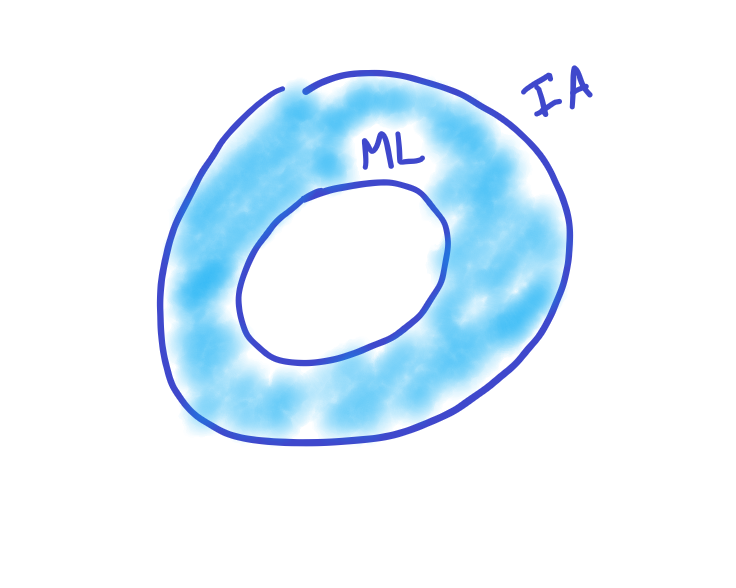
\includegraphics[width=0.3\textwidth]{img/img001.png}
  \end{center}
\end{wrapfigure}

La idea de la IA es que se tienen personas (con mucho dominio) que se juntan para resolver un problema tratando de emular de cómo se puede pensar que lo haría una persona. Lo que se haría usualmente en este caso, es fijarse de una regla que vincule las cosas que están mirando para tratar de emularlo. 

Con esto, la IA se diferencia de ML en que en IA se necesita de mucha ingeniería y de mucho conocimiento experto que está decidiendo de cómo un humano toma decisiones en un algoritmo.

De esta forma, para la IA es muy importante el conocimiento experto: tanto de quien va a generar el proceso como de quién lo programa. 

El cambio de paradigma al introducir ML, es la forma de mirar el problema, pues \textbf{no se va a querer} que un experto decida el cómo una máquina va a resolver el problema, si no que se quiere generar un algoritmo general que, a través de la experiencia, sepa cómo resolver el problema.

\begin{wrapfigure}{l}{0.3\textwidth}
  \begin{center}
    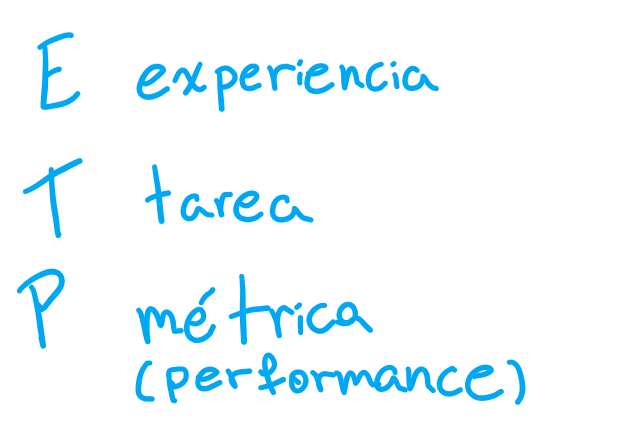
\includegraphics[width=0.25\textwidth]{img/img002.png}
  \end{center}
\end{wrapfigure}

La \emphname[Experiencia]{experiencia}, desde la perspectiva humana, es lo que permite equivocarse y permitir aprender a partir de los errores anteriores. 

La \emphname[Tarea]{tarea} es lo que se quiere resolver específicamente. Por ejemplo, dada una foto, se quiere determinar si hay un gato, o dado un texto, se quiere saber si el texto es positivo o negativo.

Por último, la \emphname[Métrica]{métrica} intenta determinar qué tan bien se está resolviendo el problema o la tarea. Sin embargo, ¿por qué cuando uno piensa en algoritmos usuales la métrica no aparece? porque usualmente evaluamos la efectividad de un modelo a partir de que si hace bien una tarea o no.

Pero cuando se pasa al paradigma de ML, lo que se va a suponer es que el algoritmo puede no estar muy bueno, y la forma de evaluar esto es a través de una métrica. Sin embargo, se tiene la promesa de que, a través de que se consiga más experiencia, el algoritmo desarrollará mejor una tarea.

Es por esto que se llama ``Aprendizaje de Máquinas'', pues es el proceso en que uno le enseña a una máquina a cómo hacer una tarea.

% La experiencia son los datos históricos, la tarea es lo que se quiere hacer y la métrica es para determinar lo ``que tan bien lo está haciendo''. Por lo usual, se quiere un algoritmo ``perfecto'' que no se equivoque, pero cuando se entra en el área de ML, vamos a tener la disposición de que el algoritmo se equivoque, y vamos a evaluar qué tan bien lo hace  a través de la métrica.

% En ML, con más experiencia, la misma tarea lo hará con mejor métrica.

\section{Machine Learning antes del Deep Learning}

Lo que nos convoca, es \emphname[]{Deep Learning} (DL), y este estará un poquito más adentro de ML

\begin{wrapfigure}{r}{0.33\textwidth}
  \begin{center}
    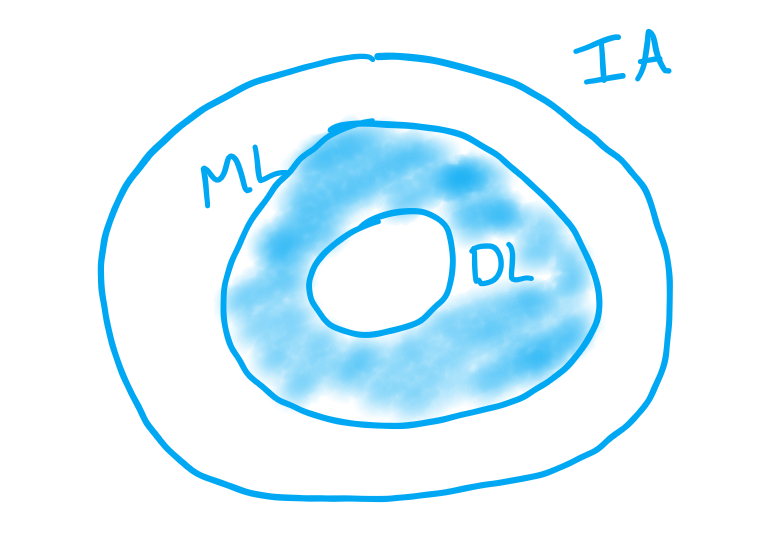
\includegraphics[width=0.3\textwidth]{img/img003.png}
  \end{center}
\end{wrapfigure}

La idea de la diferencia entre ML y DL es la siguiente: en general, los algoritmos de ML se separan en, elegir una tarea, elegir una métrica, y finalmente entregarle experiencia. Y la parte de la experiencia es crucial, pues en nuestro caso, es pasarle \textit{datos}.

Y es importante destacar en cómo hay que pasarle los datos, pues para ML, es crucial pensar en darle datos ``sencillitos'' o ``digeribles'' para el algoritmo. Típicamente se le llama las \emphname[]{características de la entrada}, esto es, la persona tiene que pensar la forma en que se representarán los datos para entregarle a los algoritmos.

Una de las ventajas de esto, es que le simplifica la vida al algoritmo, pues al no pasarle una cantidad enorme de datos, la capacidad de cómputo se ve reducida significativamente.

Y lo segundo, es que un experto en el área puede decidir cuales son los datos relevantes para resolver el problema. Esto se llama \emphname[]{extraer características} antes de pasárselo al computador.

\section{Deep Learning como ``Representation Learning''}

Lo que pasa en DL, es que el cambio de paradigma es bastante radical. La diferencia crucial es evitar precomputar las características de los datos antes de pasárselas al computador. Es decir, se intentará pasar los datos de forma muy ``cruda'' de la información. 

La promesa de DL es que si se le pasa la información muy cruda, ellos aprenderán las componentes principales (o la representación correcta de los datos) de la tarea, \textbf{a la vez que resuelven la propia tarea}. Es más, el nombre más moderno de Deep Learning, está siendo ``Representation Learning'', pues es lo que hace el modelo al fin y al cabo.

así, ya no se necesita decidir a priori cómo representar la experiencia, sino que DL lo hará de forma autónoma.

La forma de representar la experiencia se construirá como una jerarquía. Partiendo desde la información menos abstracta (lo más crudo) hasta lo más abstracta (el resultado), y cuanto más \textit{profundo}, más abstracto se hará la información. Esto justifica el nombre de \textbf{Deep} en Deep Learning. Y lo que ha mostrado la experiencia, es que a medida que se agregan más capas de abstracción exista, mejor será la métrica del algoritmo.

Sin embargo, algunas veces se querrá introducir algún tipo de sesgo para mejorar la métrica del algoritmo, pero de allí dependerá caso a caso.

\section{¿Por qué Deep Learning?}

\begin{wrapfigure}{l}{0.43\textwidth}
  \begin{center}
    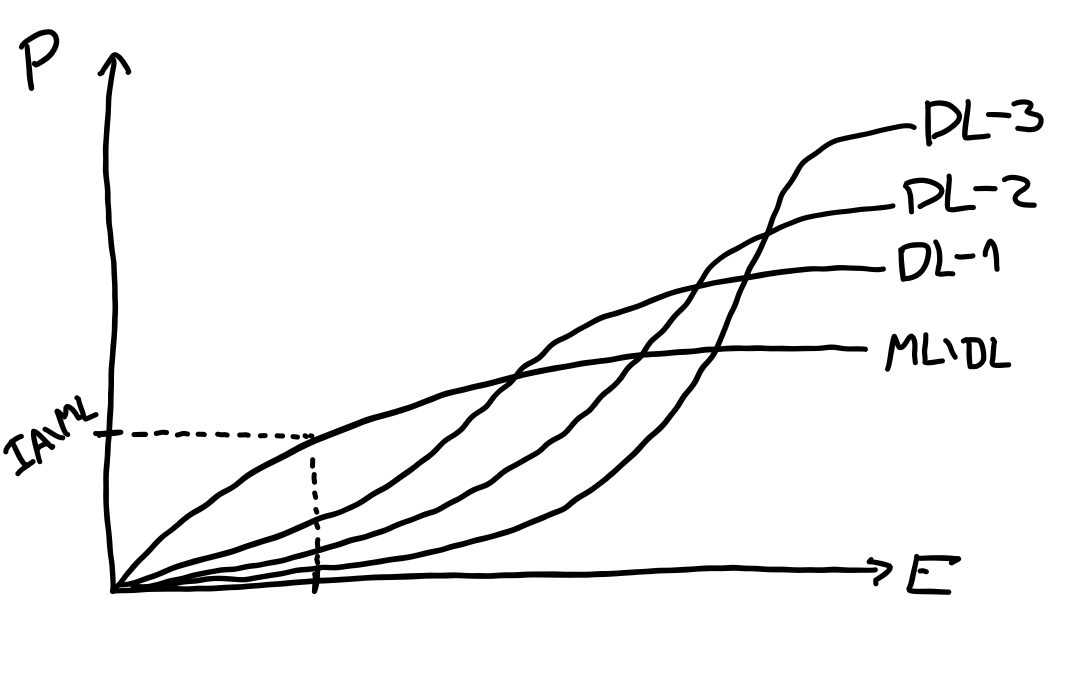
\includegraphics[width=0.4\textwidth]{img/img004.png}
  \end{center}
\end{wrapfigure}

En el gráfico se puede observar la métrica en el eje Y, y la experiencia en el eje X.

En un principio, la IA sin ML se puede ver con un desempeño medio. Se puede ver en el gráfico como IA \textbackslash ML, y que cuando se utilizan los algoritmos de ML (sin incluir los algoritmos de DL) al principio tiene un desempeño mediocre, pues no se le ha pasado suficiente experiencia. Esto sigue así hasta llegar a un límite.

Luego, con DL, se puede observar que a medida que la complejidad crece, el desempeño (la métrica) va creciendo a su vez que la experiencia crece, superando con creces a los algoritmos de ML.









\chapter{Red Neuronal}

\section{El Perceptrón}

Esta corresponde la unidad más básica de una red neuronal. Al principio, el perceptrón fue inspirada en una neurona: una unidad básica del cerebro. El comportamiento de una neurona es, al fin y al cabo, bastante simple; tan simple, que los matemáticos intentaron simularlo para comprobar si se puede obtener pensamiento inteligente. Es así cómo se ``formalizó'' el comportamiento de una neurona de forma matemática, o llevarla a un nivel computacional.
\begin{figure}
\begin{subfigure}{.47\textwidth}
    \centering
    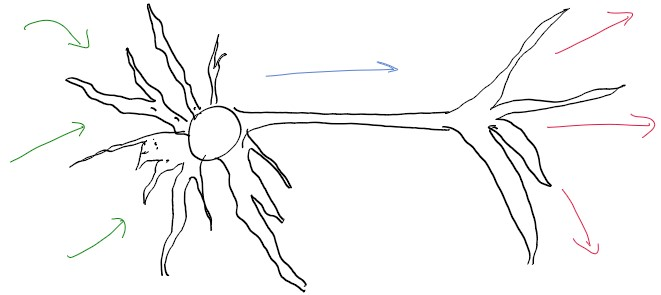
\includegraphics[width=\linewidth]{img/img005_neu_real.jpg}
    \caption{Representación de una neurona ``real''.}
    \label{fig:neu-real}
\end{subfigure}
\begin{subfigure}{.47\textwidth}
    \centering
    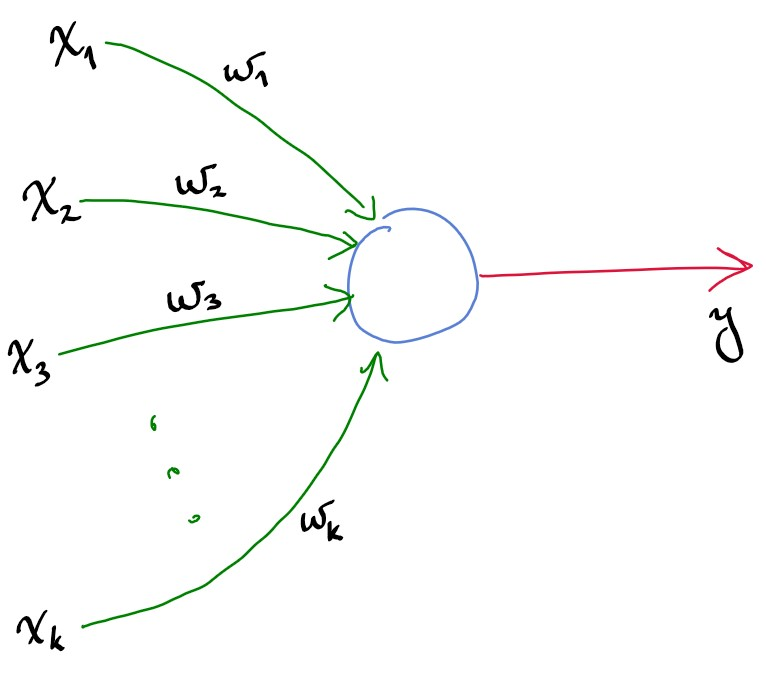
\includegraphics[width=.6\linewidth]{img/img006_neu_falsa.jpg}
    \caption{Representación del Perceptrón.}
    \label{fig:neu-virt}
\end{subfigure}
\end{figure}


\textbf{¿Cómo funciona el Perceptrón?} Tendremos la variable $u$ que representa cuánta información está recibiendo el Perceptrón. Esta variable será la suma de las variables por sus pesos (más un sesgo, a.k.a. bias)
\begin{equation}
    u = x_1 \cdot w_1 + x_2 \cdot w_2 + \ldots + x_k \cdot w_k + b
\end{equation}

Mientras que la salida del perceptrón $y$ será $u$ aplicada en alguna función, llamada \emphname[Función de Activación]{función de activación}
\begin{equation}
    y = f(u)
\end{equation}

\subsection{Funciones de activación}

A continuación se verán los distintos tipos de funciones de activación que existen:

\subsubsection*{Función escalón}
Es una función que no se ocupará mucho, sin embargo, es la más simple de todas. 
\begin{equation}
    \step(x)=
    \begin{cases}
    1 & \mbox{si } x\geq 0\\
    0 & \mbox{si } x\leq 0
    \end{cases}
\end{equation}

\missingfigure{Función escalón}

\subsubsection*{Función sigmoide}
La idea de la función sigmoide es que es como la función escalón, pero es continua y ``suave''
\begin{equation}
    \sigmoid(x) = \frac{1}{1 + e^{-x}}
\end{equation}

\missingfigure{Función sigmoide}

\subsubsection*{Función tangente hiperbólica}
Esta función de activación es cómo el símil de la función sigmoide, solo que en el régimen negativo tiende a -1 en vez de a 0. Esto se interpreta como que el perceptrón ``chupa información'' en los negativos, y ``bota información'' en los positivos.

Por mucho tiempo no se ocupó esta función de activación en los Perceptrones, principalmente porque la gente que trabaja en esta área eran muy puristas, y decían que los Perceptrones deben de parecerse lo más que se pueda a las neuronas.

Veremos más adelante que esta función de activación, en algunos casos, tiene mejor desempeño que la función sigmoide.
\begin{equation}
    \tanh(x) = \frac{e^u - e^{-u}}{e^u + e^{-u}}
\end{equation}

\missingfigure{Función Tangente hiperbólica}

\subsubsection*{Función ReLU}

Esta función viene del nombre Rectified Linear Unit.

La definición es bastante sencilla:
\begin{equation}
    \relu(x) = 
    \begin{cases}
        u & \mbox{si } u>0\\
        0 & \mbox{si } u\leq0\\
    \end{cases}
\end{equation}

\missingfigure{Función ReLU}

\subsubsection*{Función lineal}

Esta función es la más sencilla de todas, que es prácticamente la identidad.

\begin{equation}
    \lin(x) = x
\end{equation}

\missingfigure{Función lin}

\section{}
\FMG{Incluir la definición de Red Neuronal y sus capas}

\missingfigure{Dibujo de la red neuronal}

\FMG{Incluir el ejemplo de XOR}

Al final, dentro del dibujo, lo que más importante es lo que describen las ecuaciones:
\begin{eqnarray}
\bm{h} &=& f(\bm{x} W + \bm{b})\\
y &=& g(\bm{h} U + c)
\end{eqnarray}

Ahora veremos el siguiente teorema:

\begin{theorem}\namethm[UAT]{Teorema de Aproximación Universal}
Sea $F$ una función continua $[0, 1]^k \to [0, 1]$, entonces para todo $\epsilon>0$ existen $W, \bm{b}, U$ tal que $F(x) = \sigmoid(\bm{x}W + \bm{b})U$ se tiene que:
\begin{equation}
    |f(x) - F(x)|< \epsilon \quad \forall x \in [0, 1]^k
\end{equation}

\end{theorem}

Lo importante de este teorema, es que nos garantiza que tan solo basta la estructura de la red neuronal para acercarse a cualquier función continua tanto como uno quiera.

Notemos que el teorema te dice que existen los parámetros, pero no te dicen de qué dimensiones son. Existen estudios que dicen que las cotas son estúpidamente grandes, y que realmente es infactible hacer una única red neuronal ``apilando'' Perceptrones. 

Sin embargo, hay otros estudios que dicen que la efectividad aumenta conforme se van apilando Perceptrones, pero que se necesitan tantos como un crecimiento exponencial, mientras que si se agregan más capas ocultas, se necesitará un orden lineal.

Esto último nos motiva a añadir más capas ocultas, de esta forma:
\missingfigure{Red Neuronal con muchas capas}

Esta forma de red neuronal se llama MLP

La descripción matemática es la siguiente:
\begin{eqnarray}
\bm{h}^{(0)} &=& \bm{x}\\
\bm{h}^{(i)} &=& f^{(i)}(\bm{h}^{(i-1)} W^{(i)} + \bm{b}^{(i)})\\
y &=& g(\bm{h}^{(L)}U + c)
\end{eqnarray}
\end{document}